\documentclass[11pt,a4paper]{article}
\usepackage[margin=2.2cm]{geometry}
\usepackage{graphicx,booktabs,longtable,array,amsmath,amssymb,siunitx,hyperref,xcolor,tikz,float,caption,subcaption,enumitem,listings}
\usetikzlibrary{arrows.meta,positioning,shapes.geometric}
\hypersetup{colorlinks=true,linkcolor=blue!60!black,citecolor=blue!60!black,urlcolor=blue!60!black}
\sisetup{detect-all}
\lstset{basicstyle=\ttfamily\scriptsize,breaklines=true,frame=single,columns=fullflexible,keepspaces=true}
\captionsetup{font=small,labelfont=bf}
\newcommand{\um}{\si{\micro\metre}}
\newcommand{\Aum}{A/\si{\micro\metre}}
\newcommand{\ND}{\textsc{not determined from available data}}

\title{Thickness-Aware Silvaco ATLAS Model of Ultrathin W-Doped In$_2$O$_3$ (IWO) Transistors\\[4pt]
\large From literature physics to a calibrated, tested TCAD material model}
\author{IWO\_PHYSICS\_CONSTRAINED\_MODEL\_V1 --- 2--13 nm channel series}
\date{22 September 2026}

\begin{document}
\maketitle

\begin{abstract}
A single thickness-aware material description of a sputtered $\sim$2\,\% W:In$_2$O$_3$ channel was built for Silvaco ATLAS and applied to the measured bottom-gate transistors (TiN / HfO$_2$ 15 nm / Al$_2$O$_3$ 2 nm / IWO $t$ / Pd) at $V_{DS}=0.7$ V. Band gap, electron affinity, effective mass, density of states, sub-gap tail states and background donors are carried by explicit laws of thickness instead of per-device parameter sets. Twenty-seven real ATLAS launches on the local licence produced every number in this report. With one shared fitted electrostatic value (interface fixed charge $Q_f=1.73\times10^{12}$ cm$^{-2}$) and one band mobility per film, the 2.0 nm and 13.2 nm transfer curves are reproduced to 0.037 and 0.081 decades over the active region. Applied unchanged to the 6.3 nm film the model reproduces its shape but misses the threshold by 0.29 V; a single device-specific offset brings that film to 0.063 dec. Counterfactual runs with the confinement law switched off show that it is the confinement law that lets one shared charge fit both calibrated films. One-at-a-time sensitivity runs map which input controls which part of the curve. Mesh refinement passes; density-of-states level refinement reveals a 2.5\,\% systematic on the on-current, which is declared. The model is a calibrated, tested parameter extraction; it is not a predictive model of thickness scaling.
\end{abstract}

\tableofcontents
\clearpage

%======================================================================
\section{Reading guide and integrity rules}
Every simulated curve in this document is a real run of Silvaco DeckBuild 5.0.10.R + ATLAS 5.28.1.R (32-bit build) on the local licence; the run identifier (\texttt{run\_NNNN}) is printed in each figure and table and points to a directory that keeps the deck, the DeckBuild log, the logged sweep and the exported currents. Every material number carries one of ten provenance labels (Table~\ref{tab:labels}). No fit is called a measurement; no pure-In$_2$O$_3$ value is called an IWO value; no absolute PBE gap is used; no leakage floor is manufactured where the solver returns zero. Where the supplied inputs cannot fix a quantity, the text says \ND.

\begin{table}[H]\centering\small
\caption{Provenance labels used throughout.}\label{tab:labels}
\begin{tabular}{ll}\toprule
Label & Meaning\\\midrule
MEASURED\_TARGET\_DEVICE & measured on this device/process (paper, SI, schematic, workbook)\\
MEASURED\_RELATED\_MATERIAL & measured on In$_2$O$_3$ single crystal or the same process's In$_2$O$_3$\\
DFT\_PURE\_IN2O3\_PROXY & first-principles (PBE) result for pure In$_2$O$_3$, transferred to IWO\\
LITERATURE\_IWO / LITERATURE\_IN2O3\_PROXY & published value for another IWO process / for In$_2$O$_3$\\
CALCULATED & derived by an equation from labelled inputs\\
FITTED & adjusted to the measured transfer curves in ATLAS (stated stage)\\
NUMERICAL & solver/mesh setting justified by a convergence test\\
ASSUMED & no data; held fixed, listed as a limitation\\
\bottomrule\end{tabular}
\end{table}

%======================================================================
\section{The complete workflow}
Figure~\ref{fig:flow} shows the flow that was implemented, from the raw workbook to the final package. Each box corresponds to a section below.

\begin{figure}[H]\centering
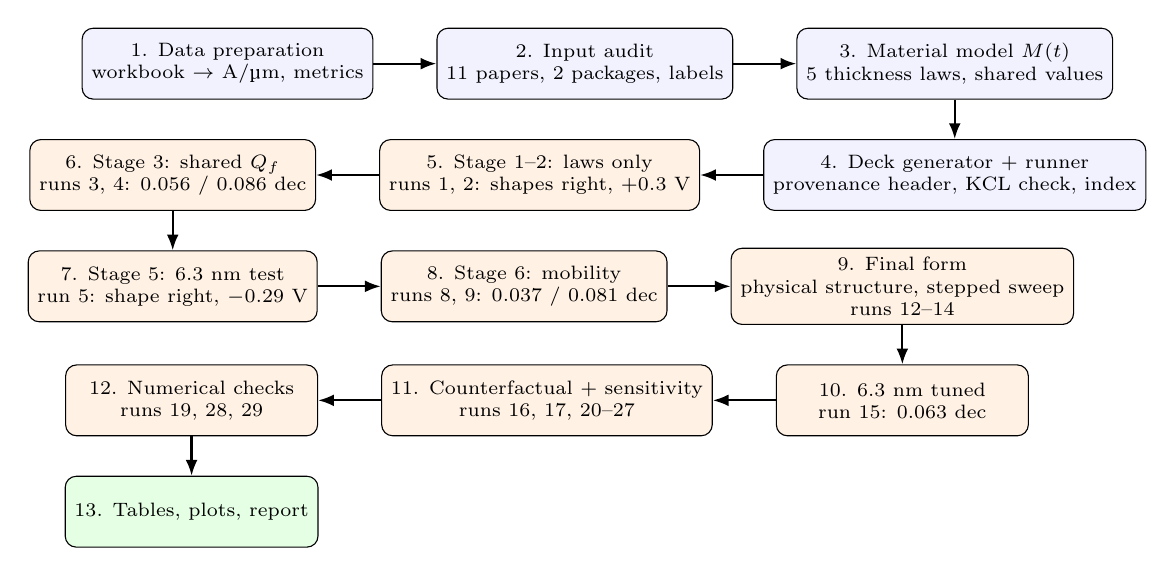
\begin{tikzpicture}[node distance=5mm and 8mm, every node/.style={font=\scriptsize},
 box/.style={draw,rounded corners,align=center,minimum width=3.2cm,minimum height=0.9cm,fill=blue!5},
 run/.style={draw,rounded corners,align=center,minimum width=3.2cm,minimum height=0.9cm,fill=orange!10},
 res/.style={draw,rounded corners,align=center,minimum width=3.2cm,minimum height=0.9cm,fill=green!10},
 arr/.style={-{Latex[length=2mm]},thick}]
\node[box](d){1. Data preparation\\workbook $\to$ A/\um, metrics};
\node[box,right=of d](a){2. Input audit\\11 papers, 2 packages, labels};
\node[box,right=of a](m){3. Material model $M(t)$\\5 thickness laws, shared values};
\node[box,below=of m](g){4. Deck generator + runner\\provenance header, KCL check, index};
\node[run,left=of g](s12){5. Stage 1--2: laws only\\runs 1, 2: shapes right, $+0.3$ V};
\node[run,left=of s12](s3){6. Stage 3: shared $Q_f$\\runs 3, 4: 0.056 / 0.086 dec};
\node[run,below=of s3](s5){7. Stage 5: 6.3 nm test\\run 5: shape right, $-0.29$ V};
\node[run,right=of s5](s6){8. Stage 6: mobility\\runs 8, 9: 0.037 / 0.081 dec};
\node[run,right=of s6](f){9. Final form\\physical structure, stepped sweep\\runs 12--14};
\node[run,below=of f](t){10. 6.3 nm tuned\\run 15: 0.063 dec};
\node[run,left=of t](c){11. Counterfactual + sensitivity\\runs 16, 17, 20--27};
\node[run,left=of c](n){12. Numerical checks\\runs 19, 28, 29};
\node[res,below=of n](r){13. Tables, plots, report};
\draw[arr](d)--(a);\draw[arr](a)--(m);\draw[arr](m)--(g);\draw[arr](g)--(s12);\draw[arr](s12)--(s3);\draw[arr](s3)--(s5);\draw[arr](s5)--(s6);\draw[arr](s6)--(f);\draw[arr](f)--(t);\draw[arr](t)--(c);\draw[arr](c)--(n);\draw[arr](n)--(r);
\end{tikzpicture}
\caption{Implemented workflow. Blue: preparation; orange: real ATLAS launches; green: reporting. Runs 6, 10 and 11 (31.8 nm attempts, one stopped run) are not part of the final set and are omitted here.}\label{fig:flow}
\end{figure}

%======================================================================
\section{The experiment}
\subsection{Device}
\begin{table}[H]\centering\small
\caption{Measured device (Januar et al.\ 2026, Sec.\ 2.1; user schematic).}
\begin{tabular}{lll}\toprule
Layer / quantity & Value & Status\\\midrule
Gate & TiN 50 nm (PVD) on n$^+$ Si & MEASURED\_TARGET\_DEVICE\\
Dielectric & HfO$_2$ $\sim$15 nm + Al$_2$O$_3$ $\sim$2 nm (ALD); Al$_2$O$_3$ touches the channel & MEASURED\_TARGET\_DEVICE\\
Channel & sputtered IWO ``$\sim$2\,\% W'', $t$ = 2.0 / 6.3 / 13.2 nm (XRR) & MEASURED\_TARGET\_DEVICE\\
Source/drain & Pd 70 nm on top of the channel & MEASURED\_TARGET\_DEVICE\\
$W/L$ & 290 / 20 \um & schematic\\
$V_{DS}$ (transfer) & 0.7 V & schematic\\
Top of channel & air, no cap & none shown\\
W composition & ``2\,\%'' undefined (at.\%, cation, mol\% WO$_3$?) & \ND\\
\bottomrule\end{tabular}
\end{table}

\subsection{Measurement and its metrics}
The workbook (SHA-256 \texttt{ce97eccd\ldots d47d12}, preserved unchanged) holds 121 points per film, $-3$ to $+3$ V in 0.05 V steps. The currents were divided once by $W=290$ \um; the simulation uses a 1 \um width so its currents are numerically in \Aum. Sweep direction, temperature, gate/source currents and the origin of the off-state plateaus are \ND.

\begin{table}[H]\centering\small
\caption{Measured metrics, extracted with the same code later applied to the simulations (Appendix~\ref{app:metrics}).}\label{tab:meas}
\begin{tabular}{lcccccc}\toprule
$t$ (nm) & $V_{th}$ (\SI{1e-9}{\Aum}) & SS$_{\min}$ (mV/dec) & SS$_{10^{-10}\ldots10^{-8}}$ & $\mu_{FE}$ (cm$^2$/Vs) & $I_{on}$ (\Aum) & off floor (\Aum)\\\midrule
2.0 & 0.66 V & 84 & 270 & 12.1 & \num{5.09e-7} & \num{4.6e-15}\\
6.3 & 0.64 V & 115 & 295 & 10.9 & \num{4.03e-7} & \num{1.5e-13}\\
13.2 & 0.08 V & 131 & 160 & 50.2 & \num{3.07e-6} & \num{6.6e-12}\\
\bottomrule\end{tabular}
\end{table}
Two facts drive the whole problem: the 6.3 nm threshold equals the 2 nm one although the 13.2 nm film is 0.58 V lower, and the apparent mobility jumps five-fold between 6.3 and 13.2 nm.

%======================================================================
\section{Physics from the literature}
\subsection{Bulk In$_2$O$_3$ and the transport-neutrality level}
In$_2$O$_3$ has a single dispersive $s$-like conduction band and a charge-neutrality level $\sim$0.4 eV \emph{above} the bulk conduction-band edge (King 2008; Robertson 2011; used by Si 2021, Lin 2022, Wang 2022). Surfaces and defects therefore tend to pin the Fermi level inside the band, the material is naturally degenerate n-type, and metal contacts are low-barrier. Bulk anchors: $m^*=0.208\,m_0$ (optical Hall, Stokey 2021), $\varepsilon_{DC}=10.55$ (single crystal) versus 8.9 for evaporated films; the target process gives, by C--V on the same stack, IWO 9.30, In$_2$O$_3$ 9.03, HfO$_2$ 19.57.

\subsection{Quantum confinement (DFT, PBE, pure In$_2$O$_3$)}
\begin{table}[H]\centering\small
\caption{Slab-minus-bulk shifts used to build the confinement law. Absolute PBE gaps (0.94 eV bulk) are never used.}
\begin{tabular}{llll}\toprule
Source & Slab & Quantity & Shift\\\midrule
Lin 2022 (ACS Nano) & 1.98 nm & $E_g^{PBE}$ 1.27 vs 0.94 eV & $+0.33$ eV\\
Lin 2022 & 0.95 nm & $E_g^{PBE}$ 1.88 eV & $+0.94$ eV\\
Lin 2022 & bulk/3.52/1.98/0.95 nm & $m^*$ 0.17/0.19/0.23/0.30 $m_0$ & $+0.02/+0.06/+0.13$\\
Si 2021 (Nano Lett.) & 1.5 nm on Al$_2$O$_3$ & $E_c$ up, $E_v$ unchanged & $\Delta E_c=+0.6$ eV\\
\bottomrule\end{tabular}
\end{table}
W raises $m^*$ and flattens the band (Januar 2026, qualitative), so the true IWO shifts are probably smaller; the uncertainty is carried as $\pm50$\,\%. No DFT of W-doped slabs exists in the inputs and none could be run here (Quantum ESPRESSO unavailable; inputs prepared).

\subsection{Sub-gap density of states}
Amorphous oxide TFTs are described by an exponential acceptor-like conduction-band tail $g_{TA}(E)=N_{TA}\exp[(E-E_c)/W_{TA}]$, a deep acceptor Gaussian, and interface states $D_{it}$. Wang 2022 measured $D_{it}\approx6.3\times10^{11}$ cm$^{-2}$eV$^{-1}$ and a bulk DOS of $3.3\times10^{20}$ cm$^{-3}$eV$^{-1}$ for ALD In$_2$O$_3$/HfO$_2$; Lin 2022 inferred $D_{it}\approx6\times10^{11}$ from a 63.5 mV/dec swing; Fan 2021 used $E_g=3.05$, $\chi=4.30$ eV for a sputtered IWO.

\subsection{The analytic framework of the target paper (Januar 2026)}
\begin{align}
I_D &= I_{blend}+I_{off},\qquad I_{blend}=\Big[(1/I_{Dc})^m+(1/I_{Dt})^m+(1/I_{Dit})^m\Big]^{-1/m} \tag{1a,b}\\
I_{Dc}&=\tfrac{W}{L}\Gamma_c V_{ov}^2,\quad I_{Dt}=\tfrac{W}{L}\Gamma_t V_{ov}^{\gamma},\quad I_{Dit}=I_{off}\exp\!\Big[\tfrac{V_G-V_{FB}}{SS/\ln 10}\Big],\quad I_{off}=\tfrac{W}{L}qD_n t_s n_{FB}\big[e^{-qV_D/kT}-1\big] \tag{1c--f}\\
N_t &= \frac{C_{ox}^2}{2\theta_t\varepsilon_s kT_t}\Big[\frac{\mu_c N_c\varepsilon_s kT}{\Gamma_t C_{ox}(\gamma-1)}\Big]^{2/\gamma},\qquad n_t\approx\theta_t N_t\exp\!\Big[\frac{E_F-E_c}{kT_t}\Big] \tag{3, 8}\\
\mu_{eff}(V_G)&=\frac{n_{free}}{n_{free}+n_{tail}+n_{it}}\,\mu_{max},\qquad \mu_{sr}(V_{ov},t)=\frac{\mu_0}{1+\theta_r V_{ov}}\Big(1-\frac{\Delta_{sr}}{t}\Big)^2 \tag{5, 6}
\end{align}
The paper reports $N_t$ rising $\sim4\times$ from 13.2 to 2 nm while $\mu_{max}$ falls from 27.4 to 5.1 cm$^2$/Vs, and $\Delta_{sr}\approx2.87$ \AA{} for IWO. Mapping into ATLAS: Eq.~(5) is not inserted, it is produced by the solver's occupation of the tail states; the roughness factor of Eq.~(6) multiplies the band mobility; the Ando roll-off $\theta_r$ is not insertable natively (Sec.~\ref{sec:limits}).

%======================================================================
\section{The material model $M(t)$}\label{sec:model}
\begin{table}[H]\centering\footnotesize
\caption{Every material input, its law, its value per film and its label. Values are those written to the decks.}\label{tab:params}
\begin{tabular}{lllcccl}\toprule
Quantity & ATLAS & Law / origin & 2.0 nm & 6.3 nm & 13.2 nm & Label\\\midrule
$\Delta E_g^{QC}(t)$ & -- & $0.921\,t^{-1.382}$ eV (fit to DFT slabs) & 0.353 & 0.072 & 0.026 & DFT proxy\\
$E_g(t)$ & EG300 & $3.05+\Delta E_g$ & 3.403 & 3.122 & 3.076 & LIT\_IWO + proxy\\
$\chi(t)$ & AFFINITY & $4.30-\Delta E_c$, $\Delta E_c=\Delta E_g$ & 3.947 & 4.228 & 4.274 & LIT\_IWO + proxy\\
$m^*(t)$ & (in $N_c$) & $0.208+0.131\,t^{-1.412}$ & 0.257 & 0.218 & 0.211 & MEAS\_REL + proxy\\
$N_c(t)$ & NC300 & $2(2\pi m^*kT/h^2)^{3/2}$ (cm$^{-3}$) & \num{3.27e18} & \num{2.55e18} & \num{2.44e18} & CALCULATED\\
$\varepsilon_r$ & PERMITTIVITY & C--V, same process & 9.30 & 9.30 & 9.30 & MEAS\_TARGET\\
$N_t(t)$ & $N_{TA}W_{TA}$ & $2\times10^{19}(2/t)^{0.75}$ cm$^{-3}$ & \num{2.00e19} & \num{8.46e18} & \num{4.86e18} & FITTED law\\
$N_{TA}(t)$ & NTA & $N_t/W_{TA}$ (cm$^{-3}$eV$^{-1}$) & \num{5.00e20} & \num{2.11e20} & \num{1.21e20} & CALCULATED\\
$W_{TA}=kT_t$ & WTA & shared & 0.040 & 0.040 & 0.040 & FITTED (shared)\\
deep acceptor & NGA & $5\times10^{16}$ at $E_c-0.6$, 0.15 eV & same & same & same & ASSUMED\\
$D_{it}$ & NGA region 2 & $3\times10^{11}$ cm$^{-2}$eV$^{-1}$ at $E_c-0.3$, 0.12 eV & same & same & same & ASSUMED\\
$N_d^{eff}(t)$ & DOPING & $2.5\times10^{17}[1+(t/20)^4]$ cm$^{-3}$ & \num{2.50e17} & \num{2.52e17} & \num{2.97e17} & FITTED law\\
$\mu_{band}(t)$ & (in MUN) & fitted per film (stage 6/8) & 18.13 & 11.69 & 61.9 & FITTED\\
roughness & (in MUN) & $(1-0.287/t)^2$ & 0.734 & 0.911 & 0.957 & LIT\_IWO\\
MUN & MUN & $\mu_{band}(1-\Delta_{sr}/t)^2$ & 13.30 & 10.65 & 59.24 & CALCULATED\\
$Q_f$ & INTERFACE QF & shared (stage 3); 6.3 nm device-specific & \num{1.73e12} & \num{8.7e10} & \num{1.73e12} & FITTED\\
$\Phi_{TiN}$ & CONTACT & 4.70 eV & same & same & same & ASSUMED\\
S/D & CONTACT & Ohmic (no work function) & -- & -- & -- & ASSUMED\\
$\sigma$, $\tau$, $N_v$ & SIG*, TAUN0, NV300 & $10^{-15}$ cm$^2$, 1 \si{\micro s}, $10^{19}$ & same & same & same & ASSUMED\\
$C_{ox}$ & -- & $\varepsilon_0/(15/19.57+2/9.0)$ nm & \multicolumn{3}{c}{\num{8.955e-7} F/cm$^2$} & CALCULATED\\
\bottomrule\end{tabular}
\end{table}

\begin{figure}[H]\centering
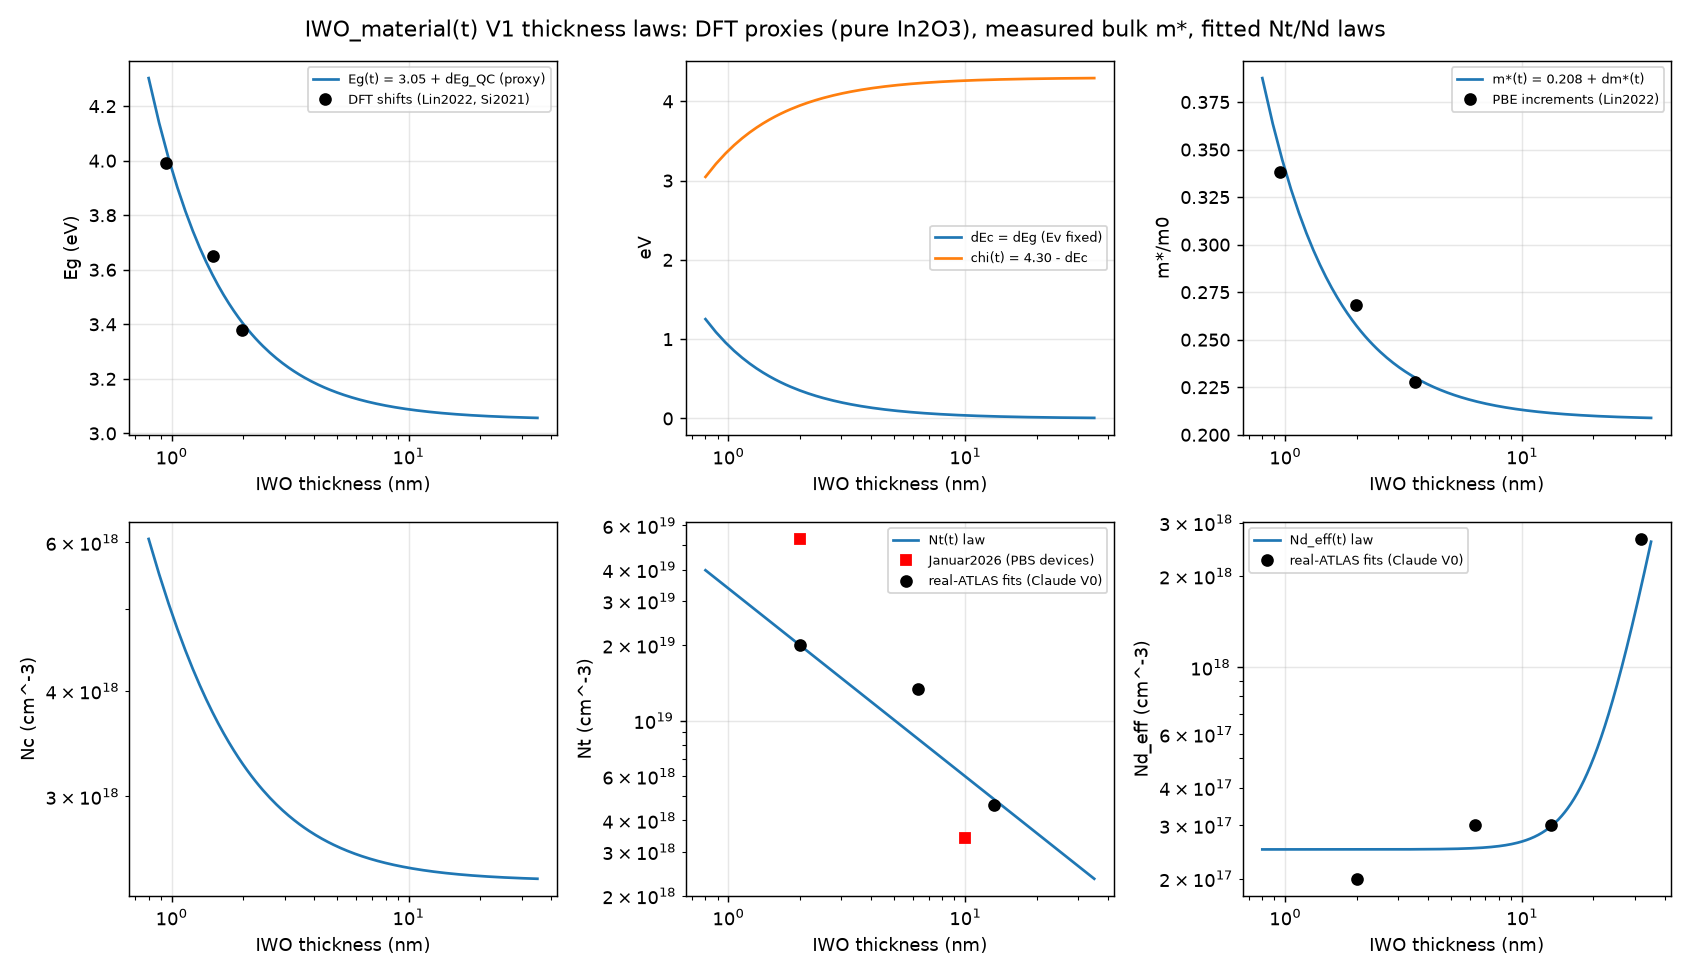
\includegraphics[width=0.95\textwidth]{figures/thickness_laws_overview.png}
\caption{The thickness laws of $M(t)$ with the evidence points they were fitted to (DFT slabs, earlier real-solver calibrations, paper trends).}
\end{figure}

\subsection{Why each term exists}
\begin{itemize}[leftmargin=*]
\item \textbf{$\chi(t)$, $E_g(t)$}: the only mechanism in the inputs that shifts the 2 nm turn-on positive relative to 13.2 nm by a physically derived amount (0.35 eV). Because the confinement is put into $E_g$, $\chi$, $m^*$ and $N_c$ explicitly (``Approach A''), no BQP or Schr\"odinger correction is enabled (it would double count).
\item \textbf{$N_c(m^*)$}: sets the Fermi level--carrier relation; the earlier calibrations used $5\times10^{18}$ with no source.
\item \textbf{Tail $N_{TA},W_{TA}$}: sets the subthreshold slope and the free/trapped partition of the induced charge, i.e.\ Eq.~(5) of the paper realised by the solver.
\item \textbf{$D_{it}$}: adds swing near its energy; kept separate from $Q_f$, which only shifts the flat band.
\item \textbf{$N_d^{eff}$}: the electrically active background donors (oxygen vacancies, hydrogen, the ionised fraction of W). It is three orders of magnitude below the W atom density and is not derived from the W content. For $t\le13$ nm it shifts $V_{th}$ by 0.01--0.07 V only.
\item \textbf{$Q_f$}: one shared value; it absorbs the unmeasured absolute $\chi$, the TiN work function and any true fixed charge, which one curve per device cannot separate. With $Q_f=0$ both calibrated films were offset by the \emph{same} 0.3 V, which is what an alignment constant looks like and a thickness-dependent $\chi$ error would not.
\item \textbf{$\mu_{band}$}: fitted last, at fixed electrostatics, to $I_{on}$; it moved $V_{th}$ by $<10$ mV, so it corrected nothing else. The 6.3$\to$13.2 nm step has no defensible law.
\end{itemize}

%======================================================================
\section{Device structure in ATLAS and the deck}
\begin{figure}[H]\centering
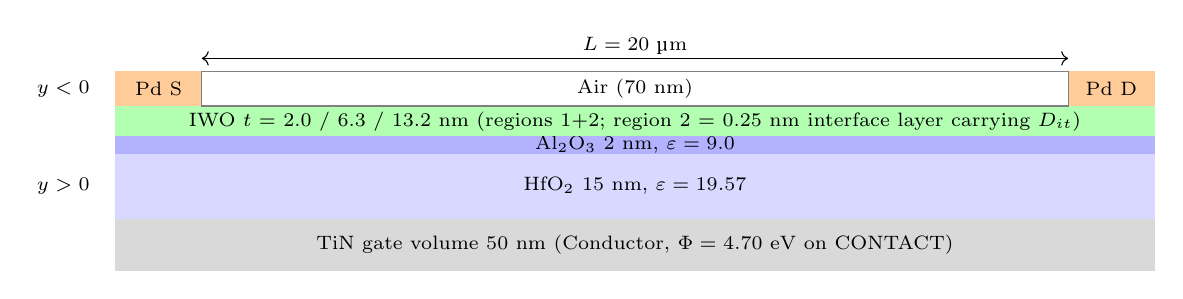
\begin{tikzpicture}[x=0.55cm,y=0.55cm,font=\scriptsize]
\fill[gray!30](0,-1.2) rectangle (24,0); \node at (12,-0.6){TiN gate volume 50 nm (Conductor, $\Phi=4.70$ eV on CONTACT)};
\fill[blue!15](0,0) rectangle (24,1.5); \node at (12,0.75){HfO$_2$ 15 nm, $\varepsilon=19.57$};
\fill[blue!30](0,1.5) rectangle (24,1.9); \node at (12,1.7){Al$_2$O$_3$ 2 nm, $\varepsilon=9.0$};
\fill[green!30](0,1.9) rectangle (24,2.6); \node at (12,2.25){IWO $t$ = 2.0 / 6.3 / 13.2 nm (regions 1+2; region 2 = 0.25 nm interface layer carrying $D_{it}$)};
\fill[orange!40](0,2.6) rectangle (2,3.4); \node at (1,3){Pd S};
\fill[orange!40](22,2.6) rectangle (24,3.4); \node at (23,3){Pd D};
\fill[white,draw=gray](2,2.6) rectangle (22,3.4); \node at (12,3){Air (70 nm)};
\draw[<->](2,3.7)--(22,3.7); \node at (12,4){$L=20$ \um}; \node at (-1.2,3){$y<0$}; \node at (-1.2,0.75){$y>0$};
\end{tikzpicture}
\caption{Physical structure used for the final runs (not to scale). MESH WIDTH = 1 \um. The reduced boundary deck used in the calibration stages replaces the metal volumes by ideal boundaries; the two representations agree to 0.1\,\% (Sec.~\ref{sec:num}).}
\end{figure}

\subsection{Structure block (2 nm deck, annotated)}
\begin{lstlisting}
go atlas
mesh width=1.0                         # 1 um -> currents in A/um
x.mesh loc=0 spac=0.3 ... loc=2 spac=0.01 ... loc=12 spac=0.7 ... loc=24 spac=0.3
y.mesh loc=-0.072 spac=0.02            # top of Air/Pd layer
y.mesh loc=-0.002 spac=0.00025         # IWO top surface, 0.25 nm through the film
y.mesh loc=-0.00025 spac=6.25e-05      # interface layer, 0.0625 nm
y.mesh loc=0 spac=6.25e-05             # IWO/Al2O3 interface
y.mesh loc=0.002 spac=0.00025          # Al2O3
y.mesh loc=0.017 spac=0.001            # HfO2
y.mesh loc=0.067 spac=0.02             # TiN volume
region num=1 user.material=IWO  x.min=0 x.max=24 y.min=-0.002   y.max=-0.00025
region num=2 user.material=IWO  x.min=0 x.max=24 y.min=-0.00025 y.max=0
region num=3 material=Al2O3     x.min=0 x.max=24 y.min=0        y.max=0.002
region num=4 material=HfO2      x.min=0 x.max=24 y.min=0.002    y.max=0.017
region num=6 material=Conductor x.min=0 x.max=24 y.min=0.017    y.max=0.067
region num=7 material=Air       x.min=0 x.max=24 y.min=-0.072   y.max=-0.002
electrode name=gate x.min=0 x.max=24 y.min=0.017 y.max=0.067
electrode name=source material=Palladium x.min=0  x.max=2  y.min=-0.072 y.max=-0.002
electrode name=drain  material=Palladium x.min=22 x.max=24 y.min=-0.072 y.max=-0.002
doping uniform n.type conc=2.50025e+17 region=1
doping uniform n.type conc=2.50025e+17 region=2
material material=IWO user.group=semiconductor user.default=silicon \
 eg300=3.40331 affinity=3.94669 permittivity=9.3 nc300=3.27444e+18 nv300=1e+19 \
 mun=13.3 mup=0.01 taun0=1e-06 taup0=1e-06
material region=3 permittivity=9.0
material region=4 permittivity=19.57
contact name=gate workfunction=4.7
models fermi srh temp=300 print
defects region=1 continuous numa=96 numd=48 nta=5e+20 wta=0.04 ntd=0 wtd=0.1 \
 nga=5e+16 ega=0.6 wga=0.15 ngd=0 egd=3.30331 wgd=0.1 sigtae=1e-15 ... siggdh=1e-15
defects region=2 continuous numa=96 numd=48 nta=5e+20 wta=0.04 ntd=0 wtd=0.1 \
 nga=1.16757e+19 ega=0.301554 wga=0.123975 ngd=0 egd=3.30331 wgd=0.1 sig...=1e-15
interface qf=1.73e+12 x.min=0 x.max=24 y.min=-0.0000001 y.max=0.0000001
method newton trap maxtraps=10 itlimit=80 climit=1e-6 ir.tol=1e-19 cr.toler=1e-17 xandrnorm carriers=1 electrons
probe name=chan_mob x=12 y=-0.001 n.mob dir=0
probe name=chan_n   x=12 y=-0.001 n.conc
solve init
save outf=equilibrium.str
solve vstep=-0.1 vfinal=-3 name=gate
solve vstep=0.1 vfinal=0.7 name=drain
log outf=transfer.log
solve vgate=-3 vstep=0.2 vfinal=-1 name=gate
solve vstep=0.05 vfinal=0.7 name=gate
save outf=near_vth.str
method newton trap maxtraps=10 itlimit=80 climit=1e-6 ir.tol=1e-19 cr.toler=5e-18 ^xandrnorm carriers=1 electrons
solve vstep=0.05 vfinal=1.5 name=gate
solve vstep=0.1 vfinal=3 name=gate
log off
save outf=final.str
extract name="IdVg" curve(v."gate",i."drain") outfile="idvg.dat"
\end{lstlisting}
Line meanings: \texttt{user.default=silicon} is only the parser template, every relevant parameter is overridden; region 2 carries the interface Gaussian ($3\times10^{11}$ cm$^{-2}$eV$^{-1}$ / 0.25 nm, moment-matched with the bulk Gaussian); \texttt{xandrnorm} with \texttt{cr.toler=1e-17} forces both update and residual norms to converge in depletion (the default accepted $10^{-15}$ \Aum{} residual glitches), and the default criterion is restored above the measured threshold; \texttt{carriers=1 electrons} drops the numerically empty hole equation (hole currents $10^{-38}$--$10^{-55}$ A in every two-carrier run). The stepped sweep solves 76 points: 0.2 V in deep depletion, 0.05 V from $-1$ V to $+1.5$ V, 0.1 V above. For 13.2 and 6.3 nm the film mesh is $t/8$ (1 nm cap), the doping, EG300, AFFINITY, NC300, MUN and NTA take the values of Table~\ref{tab:params}, and the strict criterion applies up to 0.1 V and 0.65 V respectively.

%======================================================================
\section{Calibration procedure}\label{sec:calib}
Scoring: ``active'' = measured points above $5\times$ the measured off-band median; the score is the RMS of $\log_{10}(I_{sim}/I_{meas})$ over that region in decades. Native solver zeros are counted, excluded from log residuals and never floored.

\begin{table}[H]\centering\footnotesize
\caption{Stage ledger: what was free at each stage and what each launch showed.}\label{tab:stages}
\begin{tabular}{p{4.2cm}p{1.6cm}p{2.2cm}p{7.2cm}}\toprule
Stage & Free & Runs & Outcome\\\midrule
1--2 Laws only, $Q_f=0$ & none & 0001 (2 nm), 0002 (13.2) & shapes right (SS$_{\min}$ 81/84, 146/131); both $+0.33$ / $+0.29$ V too positive; 3.93 / 1.03 dec\\
3 One shared $Q_f=1.73\times10^{12}$ ($-0.31$ V) & 1 shared & 0003, 0004 & 0.056 / 0.086 dec, $\Delta V_{th}$ $\pm0.02$ V, $I_{on}$ $-7$\,\%; one number fixes both because the offsets agreed to 40 mV\\
5 Cross-thickness test 6.3 nm & 0 & 0005 & $V_{th}$ 0.35 vs 0.64 V; shape right (SS 108 vs 115); 0.68 dec\\
5b Evidence: device-specific $Q_f$ 6.3 nm & 1 & 0007 & 0.082 dec, $I_{on}$ $+6$\,\%\\
6 Band mobility to $I_{on}$ & 1 per film & 0008, 0009 & 16.8$\to$18.13, 57.6$\to$61.9; 0.037 / 0.081 dec; $\Delta V_{th}<10$ mV\\
7 Final form (physical structure, stepped sweep) & 0 & 0012, 0013, 0014 & identical results; 0014 = 6.3 nm validation with shared parameters\\
8 6.3 nm tuned & 1 + 1 & 0015 & $Q_f$ $8.7\times10^{10}$, $\mu_{band}$ 11.69: 0.063 dec\\
\bottomrule\end{tabular}
\end{table}
Free numbers in the final model: one shared electrostatic value, one band mobility per film, one device-specific offset for 6.3 nm. Astra used 13 tuned numbers for three films, Claude V0 22+ for four.

%======================================================================
\section{Results}
\begin{table}[H]\centering\footnotesize
\caption{Final comparison, identical extraction for both curves (runs 0012, 0013, 0014, 0015).}\label{tab:final}
\begin{tabular}{llcccccc}\toprule
$t$ & run / role & $V_{th}$ exp/sim (V) & SS$_{\min}$ exp/sim & $\mu_{FE}$ exp/sim & $I_{on}$ exp/sim (\Aum) & $\Delta I_{on}$ & RMSE (dec)\\\midrule
2.0 & 0012 calibrated & 0.66 / 0.68 & 84 / 73 & 12.1 / 11.3 & \num{5.09e-7} / \num{5.09e-7} & $+0.0$\,\% & 0.037\\
13.2 & 0013 calibrated & 0.08 / 0.05 & 131 / 151 & 50.2 / 49.0 & \num{3.07e-6} / \num{3.07e-6} & $-0.0$\,\% & 0.081\\
6.3 & 0014 validation & 0.64 / 0.35 & 115 / 108 & 10.9 / 9.1 & \num{4.03e-7} / \num{5.11e-7} & $+26.8$\,\% & 0.678\\
6.3 & 0015 tuned & 0.64 / 0.65 & 115 / 111 & 10.9 / 8.4 & \num{4.03e-7} / \num{4.03e-7} & $-0.0$\,\% & 0.063\\
\bottomrule\end{tabular}
\end{table}
Simulated off currents are native zeros or $10^{-20}$ \Aum; the measured floors are not modelled, so $I_{on}/I_{off}$ is a lower bound in the simulation and is not compared in per cent.

\begin{figure}[H]\centering
\begin{subfigure}{0.49\textwidth}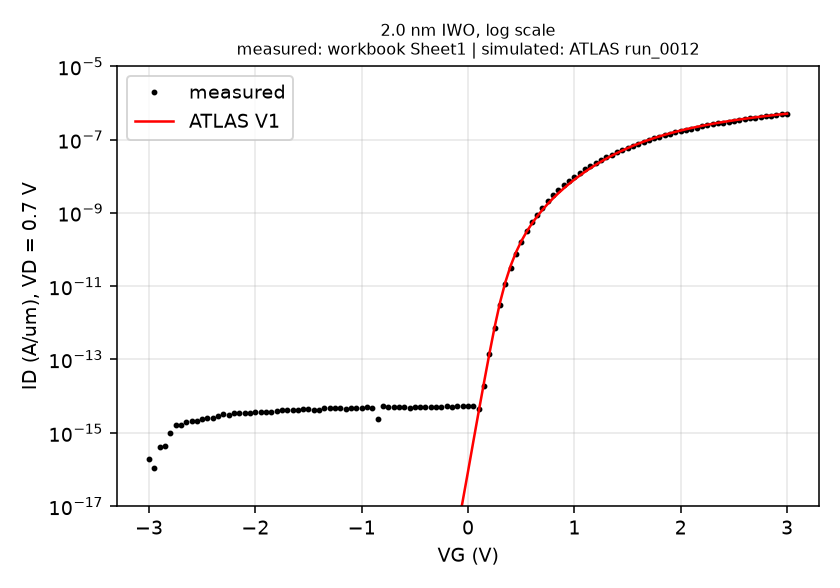
\includegraphics[width=\linewidth]{figures/2p0_overlay_log.png}\caption{2.0 nm, run\_0012}\end{subfigure}
\begin{subfigure}{0.49\textwidth}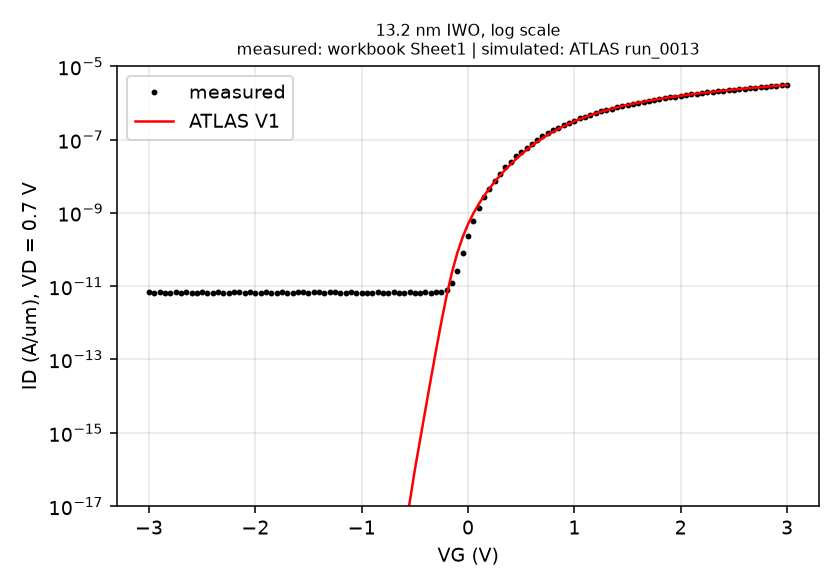
\includegraphics[width=\linewidth]{figures/13p2_overlay_log.png}\caption{13.2 nm, run\_0013}\end{subfigure}
\begin{subfigure}{0.49\textwidth}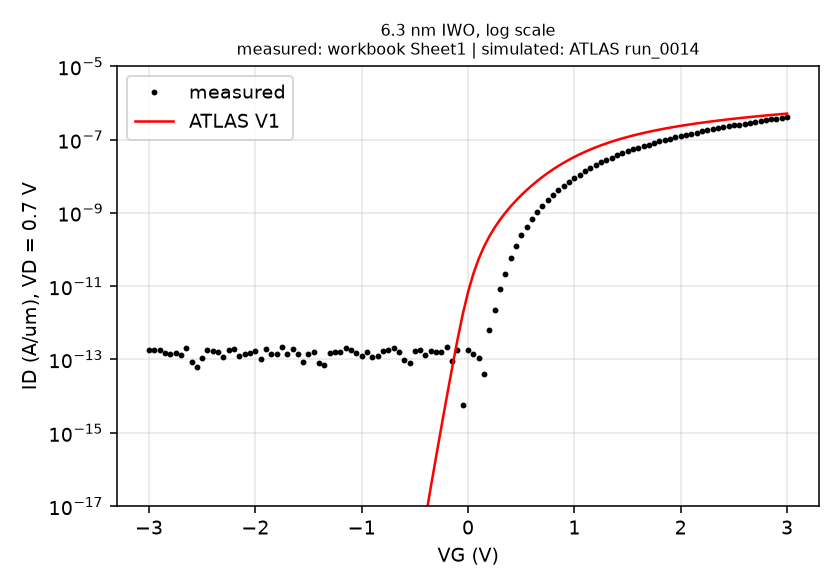
\includegraphics[width=\linewidth]{figures/6p3_validation_overlay_log.png}\caption{6.3 nm validation, shared parameters, run\_0014}\end{subfigure}
\begin{subfigure}{0.49\textwidth}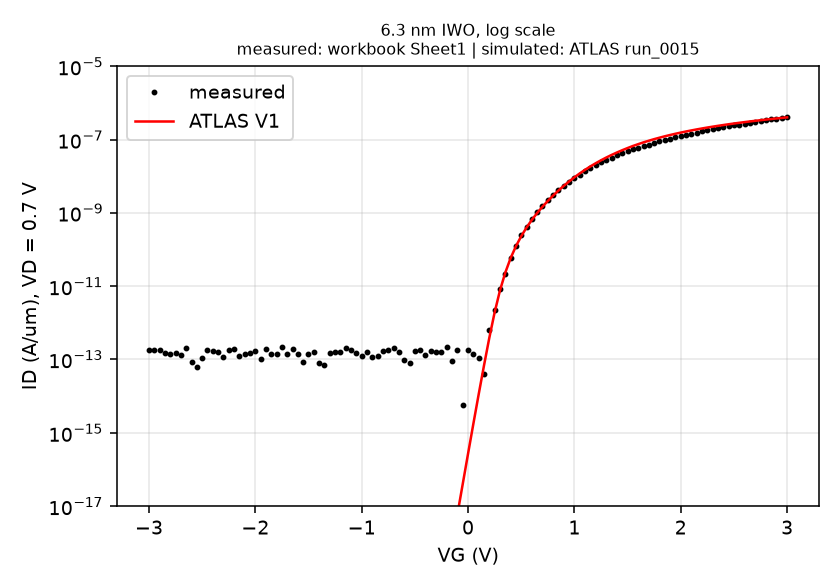
\includegraphics[width=\linewidth]{figures/6p3_overlay_log.png}\caption{6.3 nm tuned, run\_0015}\end{subfigure}
\caption{Measured (workbook) vs ATLAS transfer curves, log scale.}
\end{figure}

\begin{figure}[H]\centering
\begin{subfigure}{0.49\textwidth}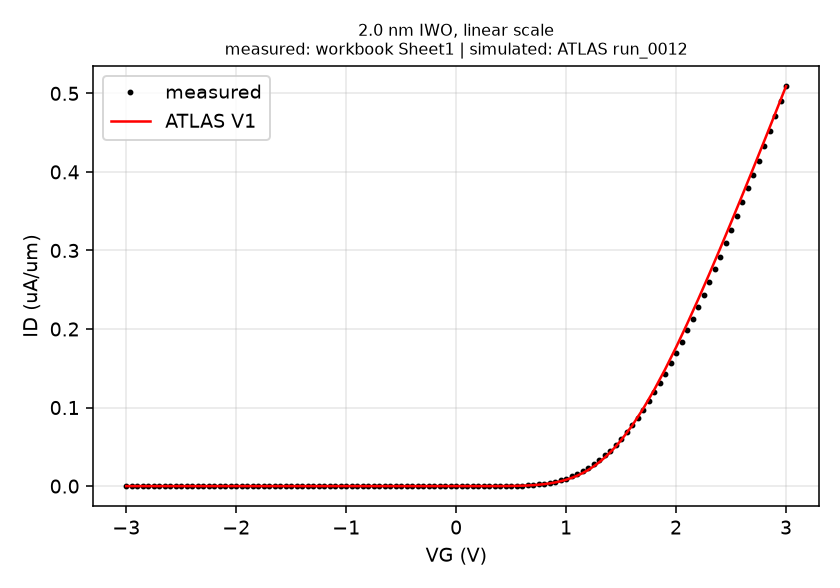
\includegraphics[width=\linewidth]{figures/2p0_overlay_linear.png}\caption{2.0 nm}\end{subfigure}
\begin{subfigure}{0.49\textwidth}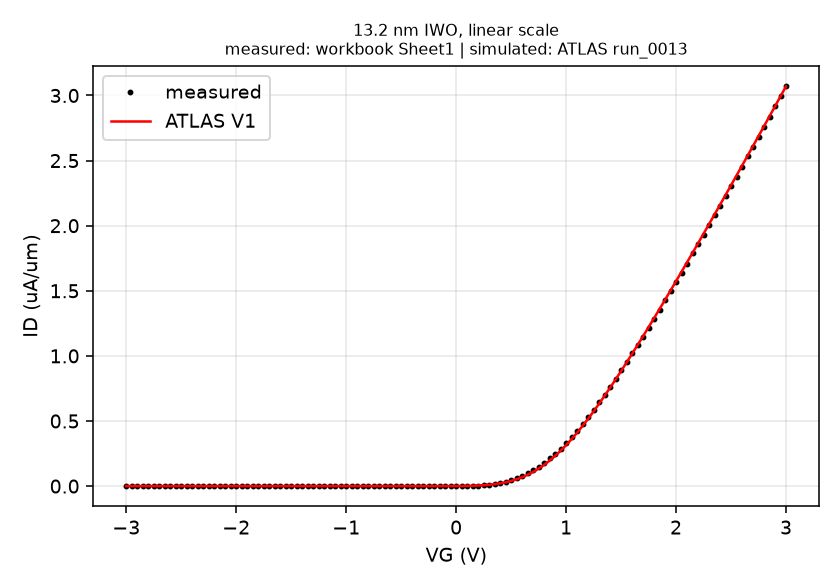
\includegraphics[width=\linewidth]{figures/13p2_overlay_linear.png}\caption{13.2 nm}\end{subfigure}
\caption{Linear-scale overlays of the calibrated films.}
\end{figure}

\begin{figure}[H]\centering
\begin{subfigure}{0.49\textwidth}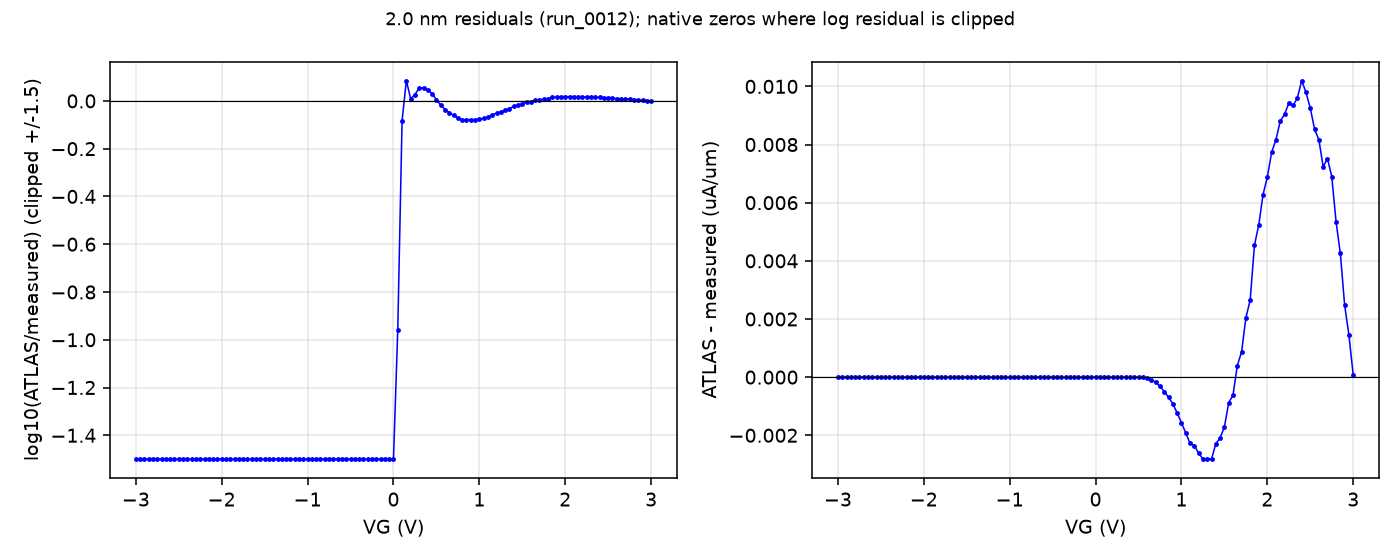
\includegraphics[width=\linewidth]{figures/2p0_residual.png}\caption{2.0 nm}\end{subfigure}
\begin{subfigure}{0.49\textwidth}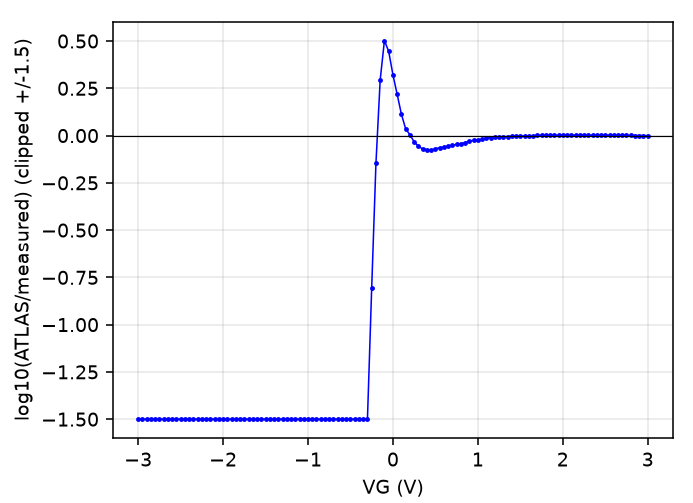
\includegraphics[width=\linewidth]{figures/13p2_residual.png}\caption{13.2 nm}\end{subfigure}
\begin{subfigure}{0.49\textwidth}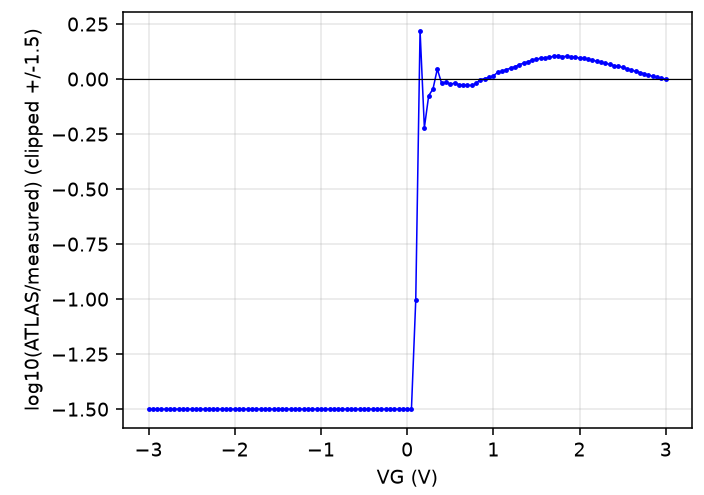
\includegraphics[width=\linewidth]{figures/6p3_residual.png}\caption{6.3 nm tuned}\end{subfigure}
\begin{subfigure}{0.49\textwidth}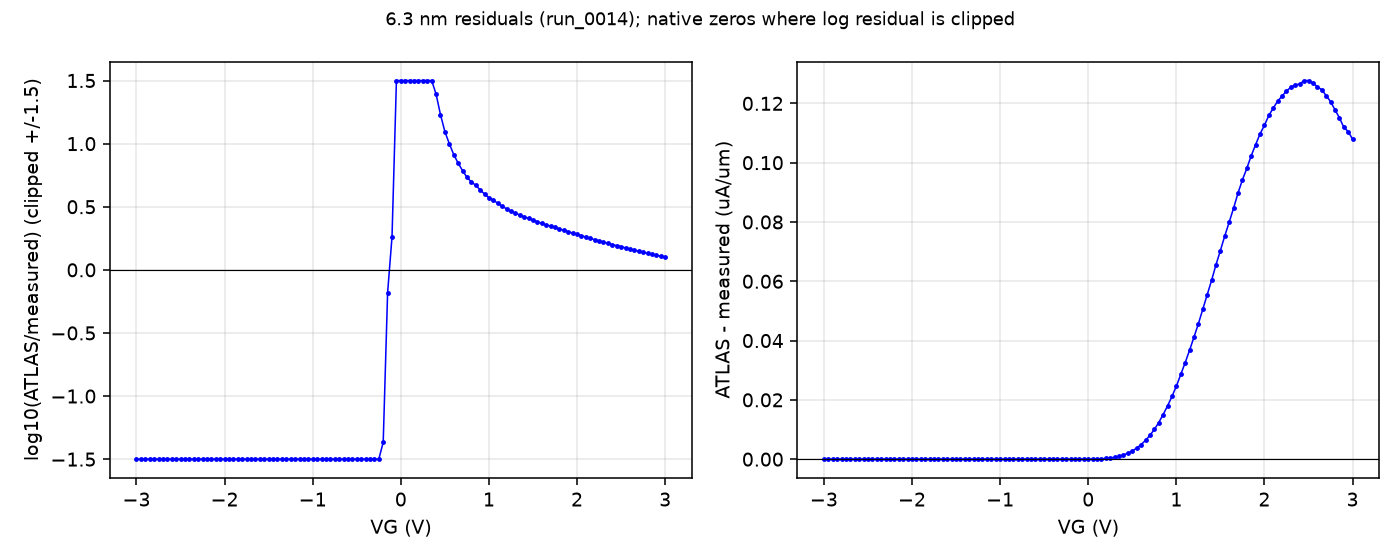
\includegraphics[width=\linewidth]{figures/6p3_validation_residual.png}\caption{6.3 nm validation}\end{subfigure}
\caption{Residuals $\log_{10}(I_{sim}/I_{meas})$ and linear differences. The 13.2 nm spike at $-0.15$ V is the point where the measured curve leaves its $6.6\times10^{-12}$ \Aum{} floor, which the simulation does not have.}
\end{figure}

\begin{figure}[H]\centering
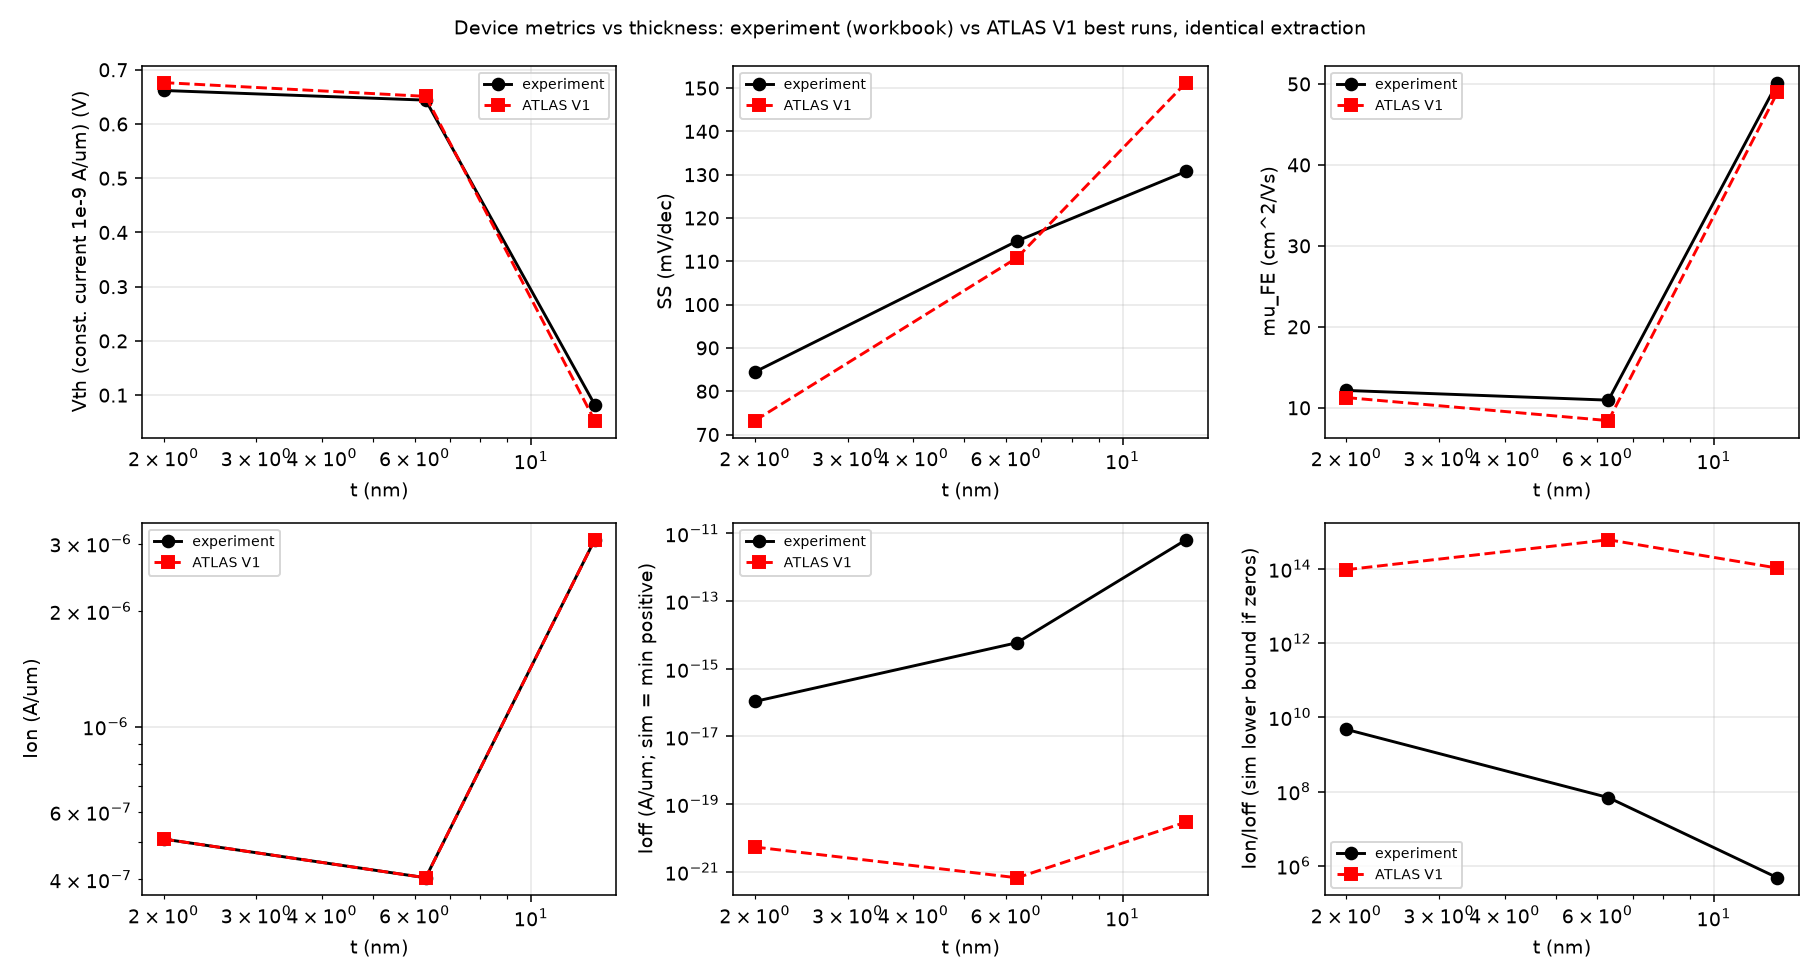
\includegraphics[width=0.95\textwidth]{figures/metrics_vs_thickness.png}
\caption{Device metrics versus thickness, experiment vs the calibrated/tuned runs, identical extraction. The off-current panel shows why $I_{on}/I_{off}$ is only a lower bound in the simulation.}
\end{figure}

\subsection{Reading the residuals}
2.0 nm: the whole active region lies within $\pm0.08$ dec, with a shallow dip near $V_G\approx1$ V (mobility peak) and a slightly steeper simulated swing (73 vs 84 mV/dec). 13.2 nm: $+0.45$ dec at the single floor-exit point, $-0.1$ dec around 0.5 V, within $\pm0.03$ dec above 1 V; simulated swing softer (151 vs 131). 6.3 nm validation: the measured curve shifted 0.29 V left with the right shape, so the $+27$\,\% on-current is an overdrive error, not a mobility error. 6.3 nm tuned: within $\pm0.1$ dec everywhere, a $+0.1$ dec hump around 1.5--2 V where the measured apparent mobility exceeds the simulated one.

\subsection{Inside the device: band diagrams, carriers, mobility}
\begin{figure}[H]\centering
\begin{subfigure}{0.49\textwidth}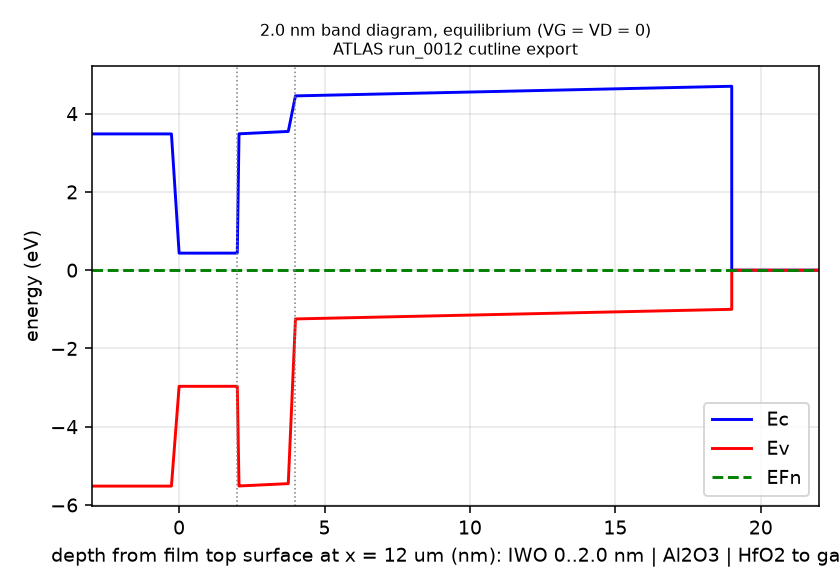
\includegraphics[width=\linewidth]{figures/2p0_band_diagram_eq.png}\caption{2.0 nm, equilibrium}\end{subfigure}
\begin{subfigure}{0.49\textwidth}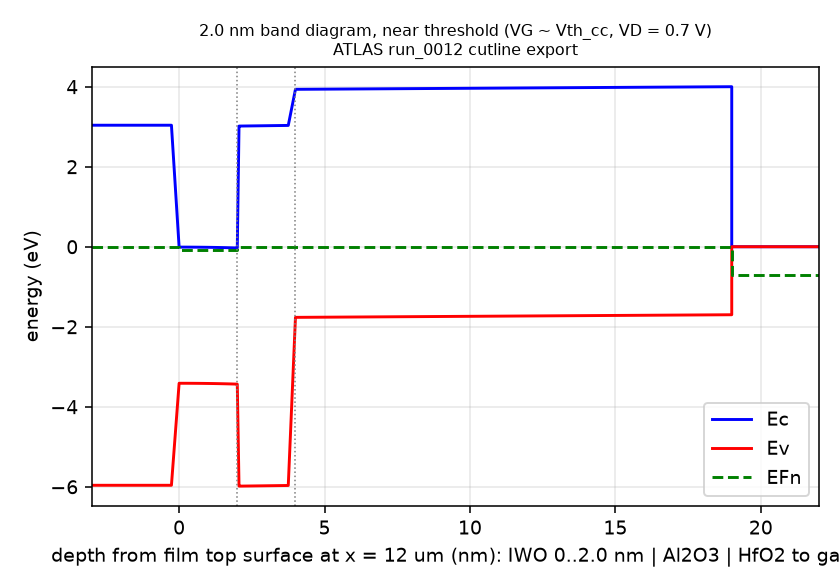
\includegraphics[width=\linewidth]{figures/2p0_band_diagram_vth.png}\caption{2.0 nm, near threshold}\end{subfigure}
\begin{subfigure}{0.49\textwidth}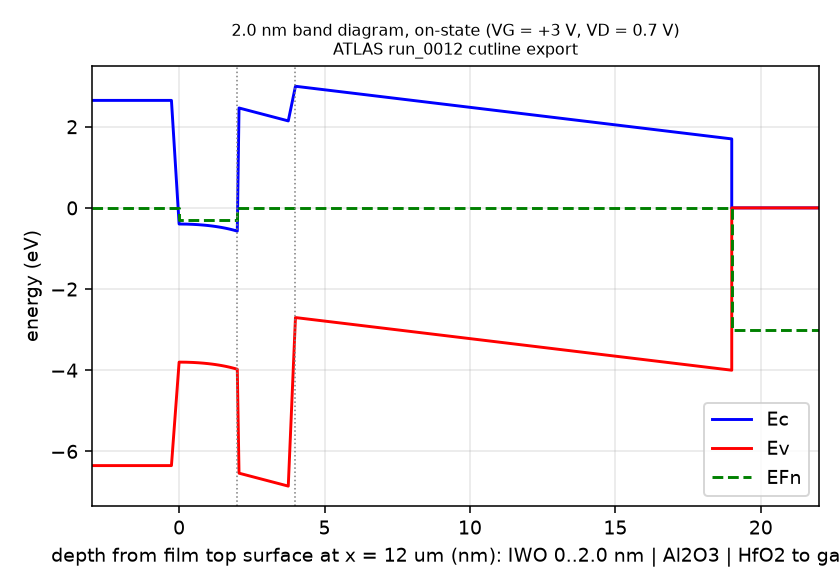
\includegraphics[width=\linewidth]{figures/2p0_band_diagram_on.png}\caption{2.0 nm, $V_G=+3$ V}\end{subfigure}
\begin{subfigure}{0.49\textwidth}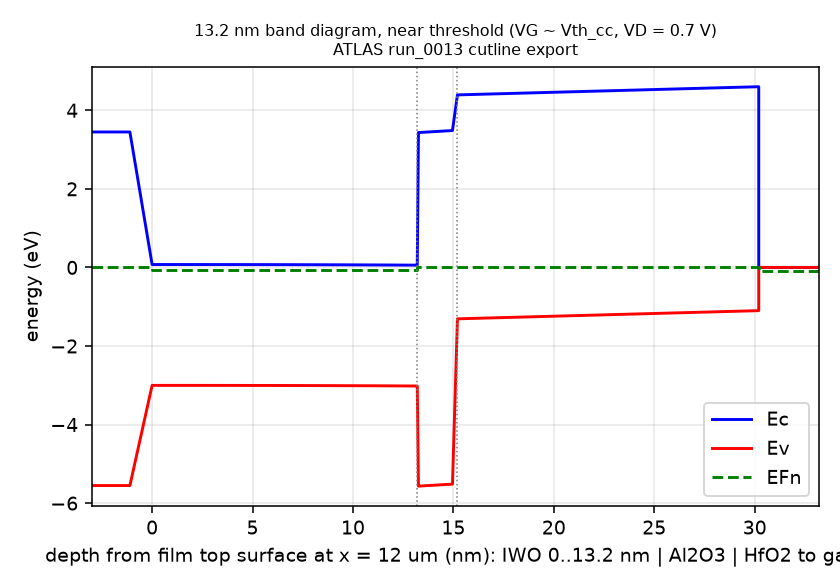
\includegraphics[width=\linewidth]{figures/13p2_band_diagram_vth.png}\caption{13.2 nm, near threshold}\end{subfigure}
\caption{Band diagrams across the stack at the channel centre (cut-line exports from the saved structures). Depth 0 = film top surface; Al$_2$O$_3$ and HfO$_2$ follow the film.}
\end{figure}

\begin{figure}[H]\centering
\begin{subfigure}{0.49\textwidth}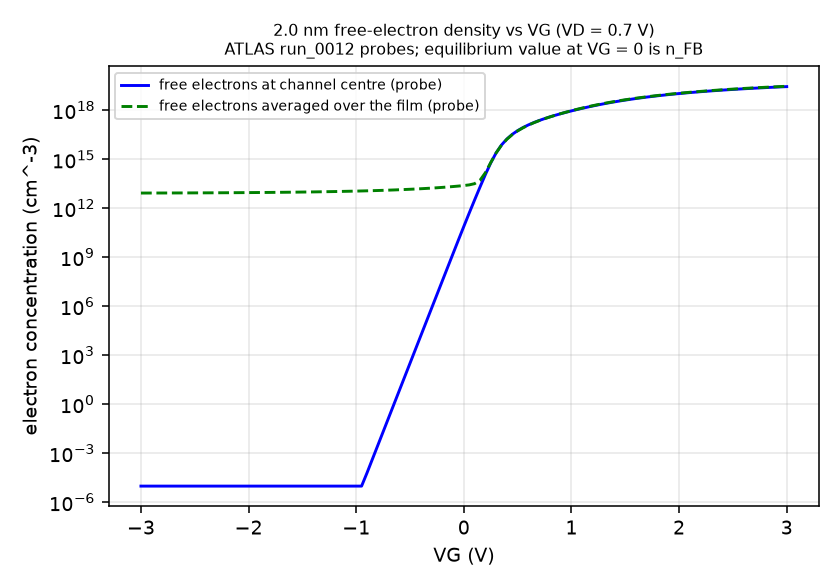
\includegraphics[width=\linewidth]{figures/2p0_electron_density_vs_vg.png}\caption{2.0 nm}\end{subfigure}
\begin{subfigure}{0.49\textwidth}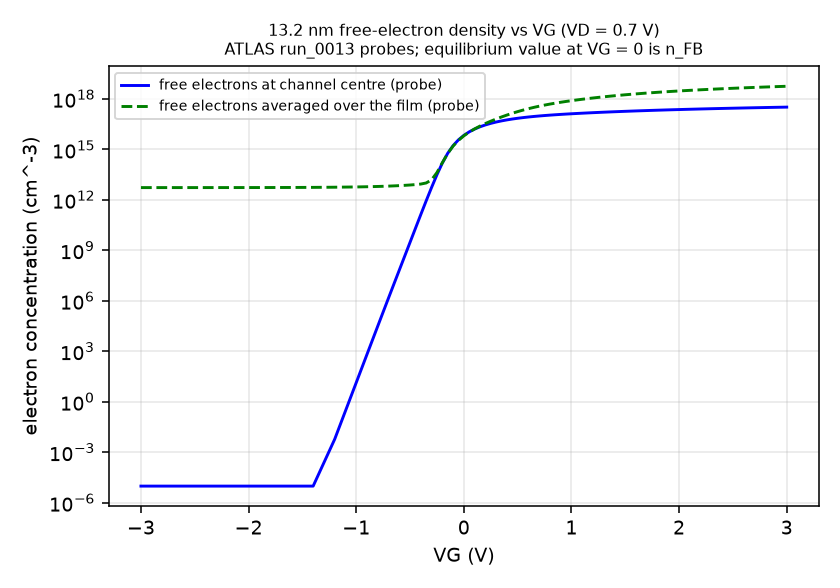
\includegraphics[width=\linewidth]{figures/13p2_electron_density_vs_vg.png}\caption{13.2 nm}\end{subfigure}
\begin{subfigure}{0.49\textwidth}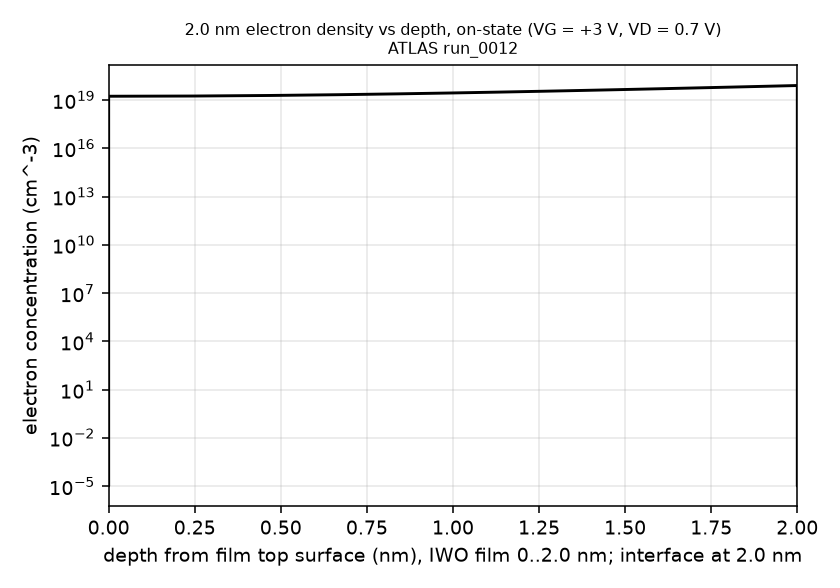
\includegraphics[width=\linewidth]{figures/2p0_electron_density_on.png}\caption{2.0 nm, on-state depth profile}\end{subfigure}
\begin{subfigure}{0.49\textwidth}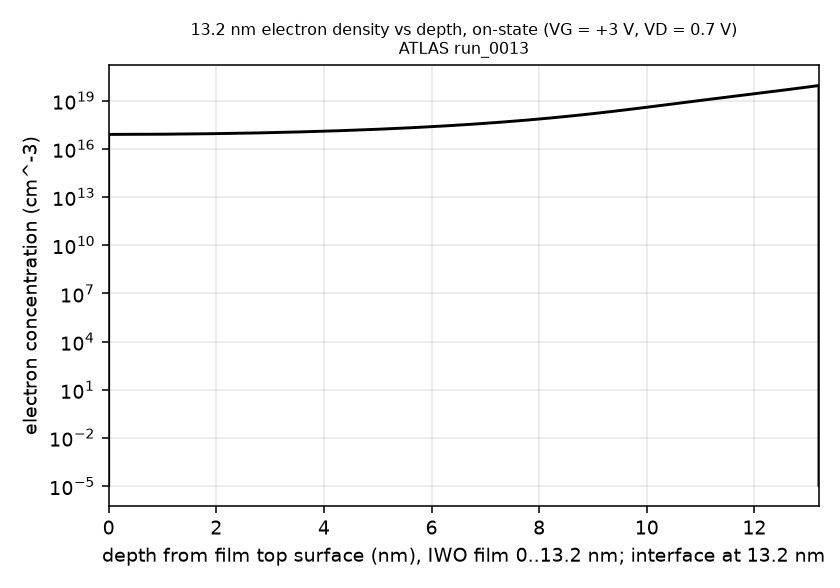
\includegraphics[width=\linewidth]{figures/13p2_electron_density_on.png}\caption{13.2 nm, on-state depth profile}\end{subfigure}
\caption{Free-electron density: versus gate bias (channel-centre probe and film average; the $V_G=0$ value is $n_{FB}$), and across the film in the on-state.}
\end{figure}

\begin{figure}[H]\centering
\begin{subfigure}{0.49\textwidth}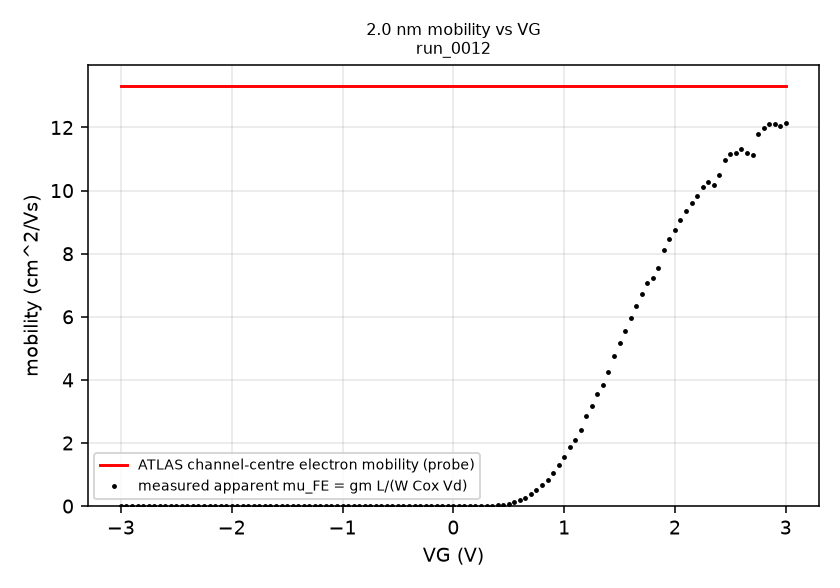
\includegraphics[width=\linewidth]{figures/2p0_mobility_vs_vg.png}\caption{2.0 nm}\end{subfigure}
\begin{subfigure}{0.49\textwidth}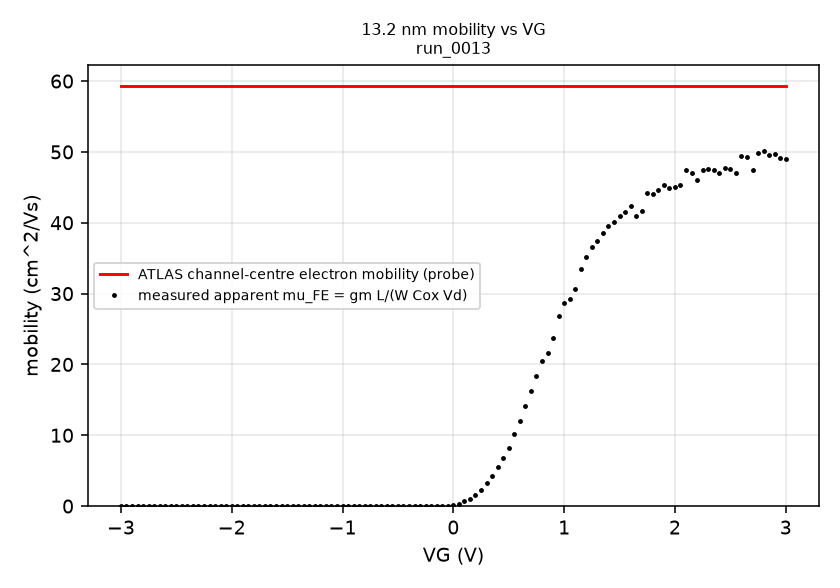
\includegraphics[width=\linewidth]{figures/13p2_mobility_vs_vg.png}\caption{13.2 nm}\end{subfigure}
\caption{Native probe mobility (constant band mobility $\times$ roughness factor) versus the measured apparent field-effect mobility $g_m L/(WC_{ox}V_D)$. The gate dependence of the apparent mobility arises from the free/trapped partition, not from a mobility model.}
\end{figure}

%======================================================================
\section{Counterfactual and sensitivity runs}\label{sec:sens}
\begin{figure}[H]\centering
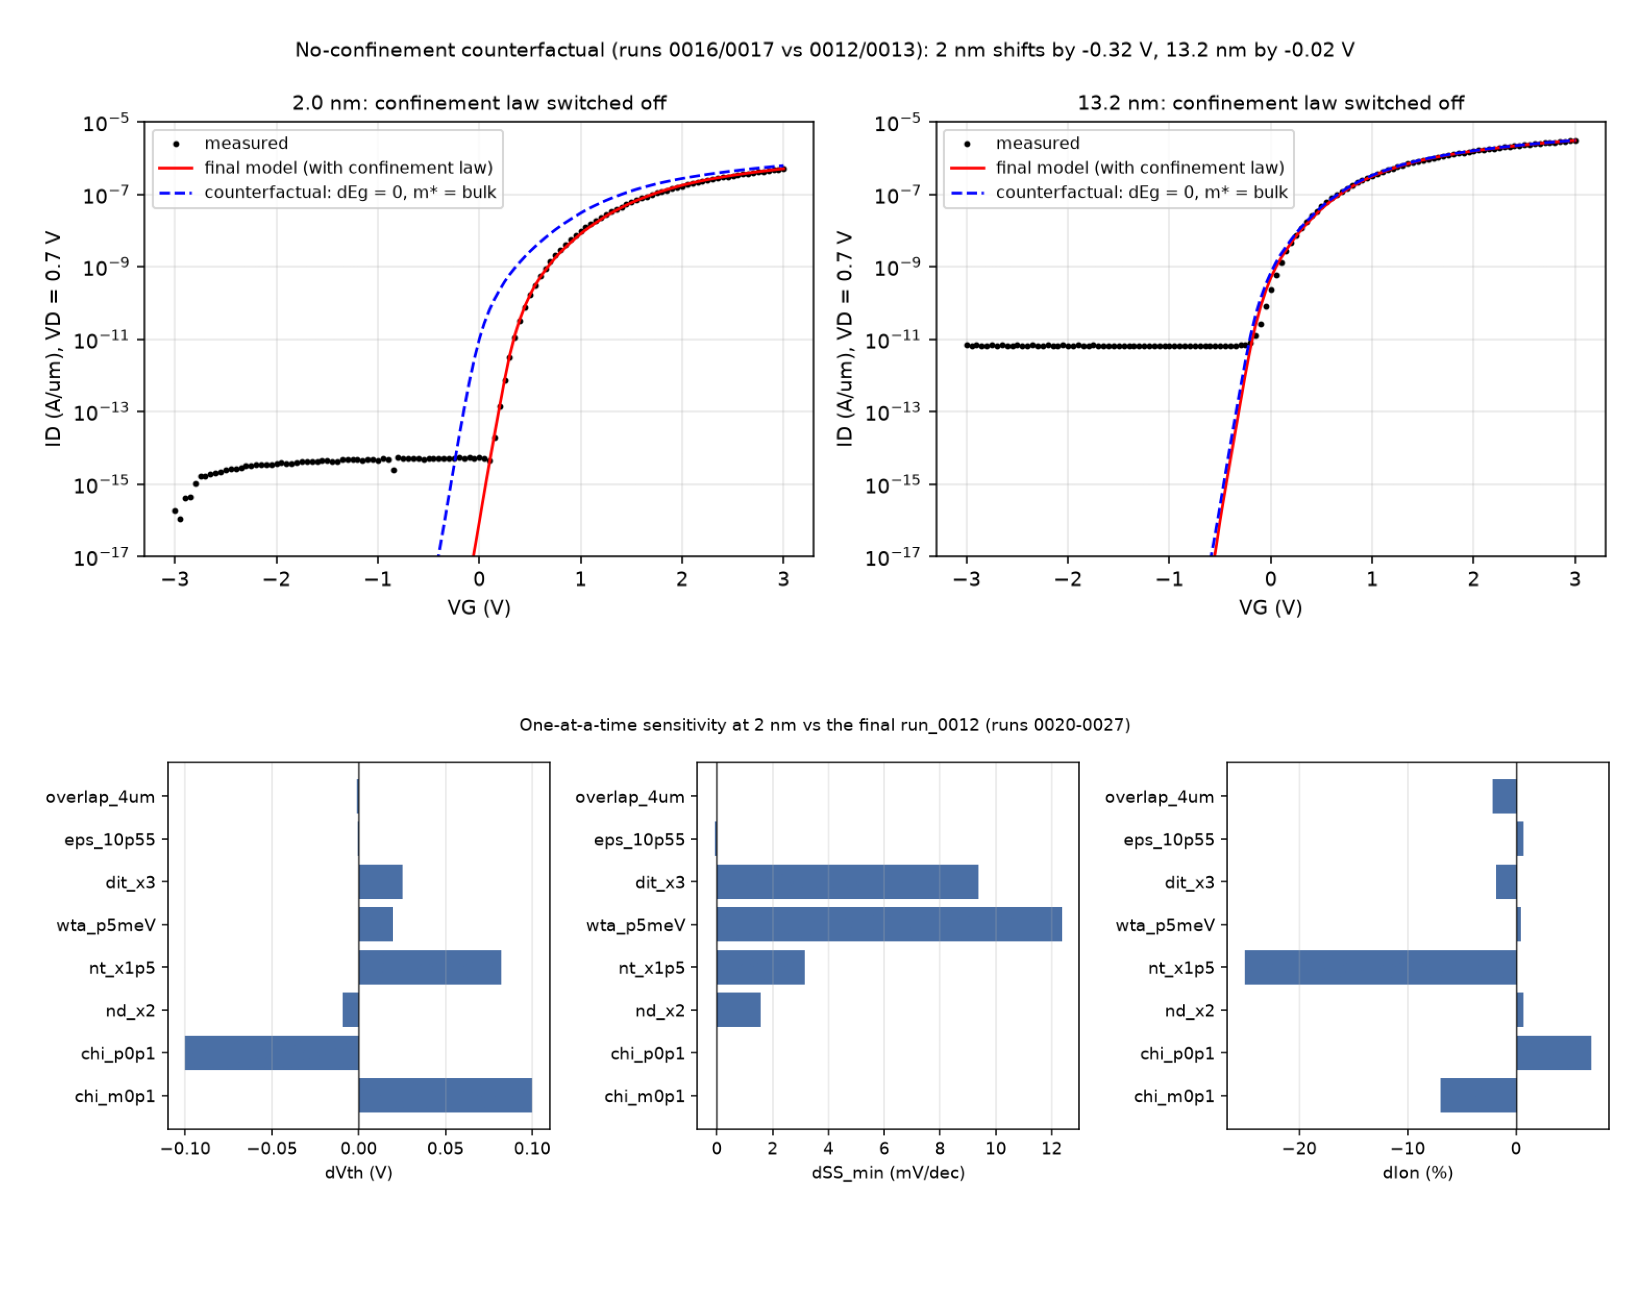
\includegraphics[width=\textwidth]{figures/sensitivity_overview.png}
\caption{Top: the confinement law switched off ($\Delta E_g=0$, $m^*=$ bulk) at 2 nm (run\_0016) and 13.2 nm (run\_0017) against the final model. Bottom: one-at-a-time perturbations at 2 nm (runs 0020--0027 vs run\_0012).}
\end{figure}

\begin{table}[H]\centering\footnotesize
\caption{Counterfactual: confinement law off, everything else at the final values.}
\begin{tabular}{lcccccc}\toprule
Film & ref & counterfactual & $\Delta V_{th}$ & $\Delta$SS$_{\min}$ & $\Delta I_{on}$ & RMSE\\\midrule
2.0 nm & 0012 & 0016 & $-0.316$ V & $+11$ mV/dec & $+21$\,\% & 0.037 $\to$ 0.846 dec\\
13.2 nm & 0013 & 0017 & $-0.023$ V & $-13$ mV/dec & $+1$\,\% & 0.081 $\to$ 0.114 dec\\
\bottomrule\end{tabular}
\end{table}
Without the law, fitting both thresholds would need fixed charges differing by $(0.316-0.023)\,C_{ox}/q=1.6\times10^{12}$ cm$^{-2}$, i.e.\ a per-device electrostatic parameter. With it, one shared value fits both. This separates ``consistent with the data'' from ``doing the work'': it is doing the work.

\begin{table}[H]\centering\footnotesize
\caption{One-at-a-time perturbations at 2 nm (each vs run\_0012; the changed input is the only difference).}
\begin{tabular}{llcccccc}\toprule
Case & run & $\Delta V_{th}$ (V) & $\Delta$SS$_{\min}$ (mV/dec) & $\Delta\mu_{FE}$ & $\Delta I_{on}$ & RMSE (dec)\\\midrule
$\chi_{bulk}-0.1$ eV & 0020 & $+0.10$ & 0 & $-0.7$\,\% & $-6.9$\,\% & 0.46\\
$\chi_{bulk}+0.1$ eV & 0021 & $-0.10$ & 0 & $+0.6$\,\% & $+7.0$\,\% & 0.36\\
$N_{d0}\times2$ & 0022 & $-0.01$ & $+1.6$ & $+0.1$\,\% & $+0.7$\,\% & 0.054\\
$N_{t2}\times1.5$ & 0023 & $+0.08$ & $+3.1$ & $-6.8$\,\% & $-25$\,\% & 0.26\\
$W_{TA}+5$ meV & 0024 & $+0.02$ & $+12.4$ & $+0.3$\,\% & $+0.4$\,\% & 0.063\\
$D_{it}\times3$ & 0025 & $+0.03$ & $+9.4$ & $-0.2$\,\% & $-1.8$\,\% & 0.098\\
$\varepsilon_{IWO}$ 9.3$\to$10.55 & 0026 & 0.00 & $-0.1$ & $+0.6$\,\% & $+0.7$\,\% & 0.037\\
overlap 2$\to$4 \um & 0027 & 0.00 & 0 & $-1.8$\,\% & $-2.2$\,\% & 0.038\\
\bottomrule\end{tabular}
\end{table}
Identifiability at 2 nm: the threshold is controlled by the band alignment ($\chi$, equivalently $Q_f$ or the work function) and weakly by the tail density; the swing by $W_{TA}$ and $D_{it}$, which are therefore separable from the electrostatics; the on-current by the tail density (free/trapped partition: $\times1.5$ in $N_t$ costs a quarter of $I_{on}$ at unchanged mobility) and by $\chi$ through the overdrive. Donors, permittivity and contact overlap are irrelevant for the 2 nm film, so the fitted electrostatics hide no donor or geometry error. Not run: gate work function (same action as $Q_f$), $m^*$ alone, and cases at 6.3 nm.

%======================================================================
\section{Numerical verification}\label{sec:num}
Pass criteria: active RMSE change $<0.01$ dec, $|\Delta V_{th}|<10$ mV, $|\Delta$SS$|<3$ mV/dec, $|\Delta I_{on}|<1$\,\%, native zeros unchanged.
\begin{table}[H]\centering\footnotesize
\caption{Convergence and consistency checks.}
\begin{tabular}{p{6.0cm}p{3.0cm}p{6.2cm}}\toprule
Check & Evidence & Result\\\midrule
Lateral mesh $\times0.5$ (2 nm, 28k nodes) & V0 runs & max 0.0046 dec, $I_{on}$ $-0.02$\,\%: PASS\\
All spacings $\times0.7$, 13.2 nm final deck (24k nodes) & 0028 vs 0013 & max 0.0032 dec, $I_{on}$ $-0.01$\,\%: PASS\\
Interface layer 0.25 $\to$ 0.125 nm & V0 runs & max 0.009 dec: PASS\\
DOS levels 96/48 $\to$ 192/96 $\to$ 384/192, 2 nm & 0019, 0029 vs 0012 & $I_{on}$ $+2.0$\,\% then $+2.5$\,\%, max 0.0125 dec, $V_{th}$/SS unchanged: \textbf{FAIL} on the 1\,\% criterion; declared as a $+2.5$\,\% systematic on all simulated $I_{on}$ and $\mu_{FE}$ (below the fit residual; a recalibration at 384/192 would lower $\mu_{band}$ by $\sim2.5$\,\%)\\
Tolerance: CR.TOLER $10^{-19}$ never converges; $10^{-17}$+XANDRNORM vs default & V0 runs & glitches removed, on-state unaffected: documented choice\\
Kirchhoff $|I_D+I_S+I_G|$ at every bias & every run & $5\times10^{-18}$..$10^{-16}$ A vs limit $\max(10^{-17}$ A, $0.1\times$ measured off-band median): PASS (one 2 nm deep-depletion point at $10^{-16}$ A exceeded an earlier limit based on a single outlier minimum; the floor was redefined and the run rescored, both records kept)\\
Electrons-only vs two-carrier & Astra rebuild & identical $I_D$; hole current $10^{-38}$--$10^{-55}$ A: PASS\\
Physical structure + stepped sweep vs reduced boundaries + per-point sweep & 0012 vs 0008, 0013 vs 0009 & $I_D$ within 0.08\,\% at 0.5 V, 0.002\,\% at 3 V: PASS\\
Width convention (WIDTH=2) & V0 & raw currents $\times2.000$, A/\um{} identical: PASS\\
6.3 nm mesh refinement & not run & OPEN\\
\bottomrule\end{tabular}
\end{table}

%======================================================================
\section{Comparison with the earlier per-device calibrations}
\begin{table}[H]\centering\footnotesize
\begin{tabular}{llll}\toprule
Item & Astra 6 & Claude V0 & V1 (this work)\\\midrule
Band parameters & $E_g$ 3.05, $\chi$ 4.30, $N_c$ $5\times10^{18}$ for all & same & $E_g(t)$, $\chi(t)$, $m^*(t)$, $N_c(t)$ from laws\\
Flat band & one shared work function & per-device $Q_f$ & one shared $Q_f$ (+1 device-specific at 6.3 nm)\\
Tail & per-device $N_{TA}$, $W_{TA}$ & per-device & $N_t(t)$ law, shared $W_{TA}$\\
$D_{it}$ & none & per-device & shared $3\times10^{11}$\\
$N_d$ & 2/1/8.9 $\times10^{17}$ & 2/3/3 $\times10^{17}$ & law\\
RMSE 2 / 6.3 / 13.2 nm (dec) & 0.033 / 0.049 / 0.049 & 0.019 / 0.048 / 0.025 & 0.037 / 0.68 (validation), 0.063 (tuned) / 0.081\\
Tuned numbers & 13 for 3 films & 22+ for 4 films & 1 shared + 1 per film + 1 device-specific\\
\bottomrule\end{tabular}
\end{table}
Robust findings common to all three: the same effective tail capacity ($\sim2\times10^{19}$ cm$^{-3}$ at 2 nm falling $\sim4\times$ by 13.2 nm), the same band-mobility step between 6.3 and 13.2 nm, and the same conclusion that intrinsic drift--diffusion cannot produce the off-state floors. V1 trades 0.03--0.06 dec of per-device accuracy for cross-thickness structure and exposes the 6.3 nm anomaly that per-device tuning had hidden.

%======================================================================
\section{Limitations and integrity statement}\label{sec:limits}
\begin{enumerate}[leftmargin=*,itemsep=1pt]
\item No DFT of the target IWO: the confinement laws are pure-In$_2$O$_3$ PBE proxies; the Quantum ESPRESSO inputs are prepared but unexecuted.
\item Absolute band alignment is not measured: $\chi_{bulk}$, the TiN work function and $Q_f$ are degenerate; only thickness differences of $\chi$ are physics. C--V or Kelvin probe per thickness would remove the degeneracy.
\item ``2\,\% W'' is undefined and never converted into a donor density.
\item Off-state floors are not modelled; their origin is \ND{} (no $I_G$/$I_S$ records).
\item Mobility: constant band mobility per film $\times$ roughness factor; the Ando roll-off is not insertable (this ATLAS ignores MOBILITY updates between SOLVE statements; its field-dependent surface models are silicon calibrations); the 6.3$\to$13.2 nm step has no law.
\item The 6.3 nm film contradicts every monotonic thickness law (its threshold equals the 2 nm one); the shared model misses it by 0.29 V; the tuned run shows one electrostatic number is all it misses; the cause is \ND.
\item $D_{it}$, capture cross sections, lifetimes, $N_v$ and the deep Gaussian are assumed and not identifiable from DC curves.
\item Quasi-2D sub-band quantisation is not represented (3-D $N_c$ with a confinement-corrected mass).
\item DOS-level discretisation leaves a $+2.5$\,\% systematic on $I_{on}$.
\item Calibration, not validation: one curve per device at one $V_D$ and temperature; the only out-of-sample test (6.3 nm) failed on the threshold.
\end{enumerate}
\textbf{Integrity.} No material parameter or source was invented; no fit is called a measurement; the W content was not treated as donors; proxies are labelled; no PBE gap is used as an experimental gap; the fitted $Q_f$ was shown to be a common offset and not a thickness patch; mobility was fitted last at fixed electrostatics; no ATLAS run, DFT run or convergence test is fabricated; no leakage was manufactured; ``exact match'' is not claimed; the model is not called predictive.

%======================================================================
\section{Publication-readiness statement}
The package is publication-ready as a calibrated, thickness-resolved TCAD parameter extraction for the 2, 6.3 and 13.2 nm devices (0.037 / 0.063 / 0.081 dec) with one shared electrostatic offset, one documented device-specific offset for the 6.3 nm film, a documented negative out-of-sample result for that film under the shared laws, a counterfactual test of the confinement law and a sensitivity/identifiability map. It is not a predictive model of thickness scaling. What would make it predictive: C--V per thickness, a second bias or temperature per device, DFT of W-doped slabs, TLM for the contacts, gate-current records for the off state.

%======================================================================
\appendix
\section{Launch index}
\begin{longtable}{lllp{7cm}}\toprule
Run & $t$ (nm) & Label & Outcome\\\midrule\endhead
0001 / 0002 & 2.0 / 13.2 & laws only & offsets $+0.33$ / $+0.29$ V\\
0003 / 0004 & 2.0 / 13.2 & + shared $Q_f$ & 0.056 / 0.086 dec\\
0005 & 6.3 & shared parameters (prediction) & 0.678 dec, $V_{th}$ $-0.29$ V\\
0007 & 6.3 & device-specific $Q_f$ (evidence) & 0.082 dec\\
0008 / 0009 & 2.0 / 13.2 & $\mu_{band}$ 18.13 / 61.9 & 0.037 / 0.081 dec\\
0012 / 0013 & 2.0 / 13.2 & FINAL: physical structure, stepped sweep & 0.037 / 0.081 dec\\
0014 & 6.3 & FINAL validation, shared parameters & 0.678 dec\\
0015 & 6.3 & FINAL tuned & 0.063 dec\\
0016 / 0017 & 2.0 / 13.2 & no-confinement counterfactual & $V_{th}$ $-0.316$ / $-0.023$ V\\
0018 & 13.2 & mesh $\times0.7$ & timed out at 900 s (rerun as 0028)\\
0019 / 0029 & 2.0 & DOS 192/96 / 384/192 & $I_{on}$ $+2.0$ / $+2.5$\,\%\\
0020--0027 & 2.0 & one-at-a-time cases & Sec.~\ref{sec:sens}\\
0028 & 13.2 & mesh $\times0.7$, 1500 s & max 0.0032 dec: PASS\\
\bottomrule\end{longtable}

\section{Metric definitions}\label{app:metrics}
$V_{th}$: gate voltage where $I_D=10^{-9}$ \Aum, log-linear interpolation. SS$_{\min}$: minimum over 0.2 V windows of $dV_G/d\log_{10}I_D$, restricted to currents above $5\times$ the \emph{measured} off-band median of the same film (applied to the simulation too, so both are evaluated over the same range) and below 1\,\% of $I_{on}$. SS$_{10^{-10}\ldots10^{-8}}$: average slope between those crossings. $\mu_{FE}=g_{m,\max}L/(WC_{ox}V_D)$, $L=20$ \um, $W=1$ \um, $C_{ox}=8.955\times10^{-7}$ F/cm$^2$, $V_D=0.7$ V. $I_{on}=I_D(+3$ V$)$. Active-region RMSE: RMS of $\log_{10}(I_{sim}/I_{meas})$ over measured points above $5\times$ the off-band median.

\section{Reproduction}
\begin{lstlisting}
python scripts/material_laws.py
python scripts/build_iwo_decks.py
python scripts/run_atlas.py --thickness 2    --label rerun --override traps.fixed_interface_charge_Qf_cm2.value=1.73e12 --override "thickness_laws.mu0_cm2Vs.mu_band_fitted[2.0]=18.13"
python scripts/run_atlas.py --thickness 13.2 --label rerun --override traps.fixed_interface_charge_Qf_cm2.value=1.73e12 --override "thickness_laws.mu0_cm2Vs.mu_band_fitted[13.2]=61.9"
python scripts/run_atlas.py --thickness 6.3  --label tuned --override traps.fixed_interface_charge_Qf_cm2.value=8.7e10  --override "thickness_laws.mu0_cm2Vs.mu_band_fitted[6.3]=11.69"
python scripts/sensitivity_analysis.py --thickness 2 --cases no_confinement chi_m0p1 nd_x2 --vstep 0
python scripts/compare_experiment_simulation.py; python scripts/plot_results.py; python scripts/make_provenance_tables.py
\end{lstlisting}

\section{References}
\begin{enumerate}[leftmargin=*,itemsep=0pt]\small
\item M. Januar, Z.-F. Luo, K.-C. Liu, M.-H. Lee, Small Structures 7, e202500807 (2026). Stack, Eqs.\ (1)--(9), $N_t$/$T_t$, $\Delta_{sr}$.
\item M. Si et al., Nano Lett.\ 21, 500 (2021). CNL 0.4 eV above $E_c$; $\Delta E_c\approx0.6$ eV at 1.5 nm.
\item Z. Lin et al., ACS Nano 16, 21536 (2022). PBE gaps and masses of In$_2$O$_3$ slabs; $D_{it}$ $6\times10^{11}$.
\item Z. Wang, Z. Lin, M. Si, P. D. Ye, Front.\ Mater.\ 9, 850451 (2022). $D_{it}$, bulk DOS of ALD In$_2$O$_3$/HfO$_2$.
\item M. Stokey et al., J. Appl.\ Phys.\ 129, 225102 (2021). $\varepsilon_{DC}$ 10.55, $m^*$ 0.208 $m_0$.
\item H. Kim et al., Appl.\ Phys.\ Lett.\ 125, 173507 (2024). Thickness trend of IWO traps.
\item M. Si et al., Nature Electronics 5, 164 (2022). Contacts/CNL.
\item N. Pandey et al., IEEE TED 72, 2381 (2025); X. Wang et al., IEEE TED 72, 2390 (2025); K. Anusha, A. Dwivedi, Meas.\ Sens.\ 36, 101391 (2024): context.
\item W.-T. Fan et al., Nanomaterials 11, 3070 (2021): $E_g$ 3.05 / $\chi$ 4.30 priors (metadata to verify).
\item P. D. C. King et al., PRL 101, 116808 (2008); J. Robertson, S. J. Clark, PRB 83, 075205 (2011); T. Ando, A. Fowler, F. Stern, RMP 54, 437 (1982); I. Hamberg, C. Granqvist, JAP 60, R123 (1986) (cited, not supplied).
\item Silvaco ATLAS User's Manual 5.28.1.R; DeckBuild User's Manual 5.0.10.R (installed copies).
\end{enumerate}
\end{document}
